\subsection{Scenarios}
\subsubsection*{A new user subscribes to the platform}
\begin{enumerate}
    \item An athlete lands on the website's landing page for the first time. After browsing the home screen and viewing the services offered by the app, they decide to sign up.
    \item The user clicks the “Sign Up” button, which redirects them to the registration page.
    \item At this point, the user must decide whether to register using their own credentials (email and password) or to use an OAuth authentication method, logging in with an account from another service.
    \item After filling in the required fields, the user is taken to the second screen of the registration flow, where they are asked to provide additional information needed to calculate performance metrics, such as weight, height, age, etc.
    \item Finally, the user is successfully registered and is redirected to the application's main screen.
\end{enumerate}
\subsubsection*{A user records an activity}

\begin{enumerate}
    \item When a user wants to record an activity, they must go to the “Record Trip” panel.
    \item From there, in the “Automatic” section, they simply need to press the play button: the app will start recording GPS data and storing the route and detected potholes.
    \item Once the route is completed, pressing the stop button will end the recording.
    \item At this point, the user will be asked to verify whether the obstacles detected by the application are actually present or are false positives, and to confirm the condition of the path.
    \item The system automatically analyzes the recorded GPS trace to check if it matches an existing public path.
    \item If a match is found, the activity is associated with that path, and the validated information is automatically merged with the existing data.
    \item If no match is found, a prompt will ask the user whether they want to publish the new route or keep it private.
\end{enumerate}

\subsubsection*{A user creates a path manually}
\begin{enumerate}
    \item The user logs into the platform using their credentials.
    \item Once authenticated, the user accesses the “My Paths” section of their profile.
    \item The user selects the “Add Path” option to start creating a new route.
    \item The system opens a dedicated page for creating the path.
    \item The user enters the required information, including:
        \begin{itemize}
            \item The name of the path,
            \item The positions that compose the path,
            \item The condition of the path,
            \item The presence of any obstacles or issues present along the route.
        \end{itemize}
    \item After completing the input, the user confirms the creation of the path.
    \item The system saves the data and displays a confirmation message.
    \item The system also offers the user the option to make the path public, so it can be shared with the community.
    \item The newly created path is displayed in the “My Paths” section of the user’s profile.
\end{enumerate}
\subsubsection*{A user searches for a path}
\begin{enumerate}
    \item The user can choose to:
        \begin{itemize}
            \item log in with their account, or
            \item use the platform without authentication.
        \end{itemize}
    \item From the home page, the user enters the starting point and the desired destination in the search bar.
    \item The system receives the request and queries its database of published paths.
    \item The system processes the available options and calculates a score for each path based on:
        \begin{itemize}
            \item the condition of the segments,
            \item the freshness of the information,
            \item the effectiveness of the route in connecting the selected points.
        \end{itemize}
    \item The system displays the results on the map, ordered in descending order of score.
    \item The user reviews the results and can select a specific path to view more details.
    \item The system displays detailed information for the selected path, such as:
        \begin{itemize}
            \item total distance,
            \item estimated travel time,
            \item overall condition of the route.
        \end{itemize}
\end{enumerate}
\subsubsection*{User publishes a path}
\begin{enumerate}
    \item The user accesses the BBP system and opens the “My Paths" section.
    \item The system displays the list of paths associated with the user, indicating for each one, among other properties, its status (private or public).
    \item The user selects a private route and, using the appropriate button, requests its publication.
    \item Upon receiving the publication request, the system asks the user to confirm additional information related to the route:
        \begin{itemize}
            \item In the case of manually created routes, the user can review and, if necessary, modify the additional information previously entered during creation.
            \item In the case of automatically generated routes, the user must confirm or correct the acquired information (if not already done) and may add further details manually.
        \end{itemize}
    \item Once the review is complete, the user confirms the publication of the route.
    \item The system verifies the data consistency, assigns a unique identifier to the route, and makes it available to the community within the search and browsing functionality.
    \item The system notifies the user of the successful publication and updates the route status from private to public.
\end{enumerate}
\subsubsection*{User modifies the additional information related to a route}
\begin{enumerate}[label=\arabic*.]
    \item The user accesses the Best Bike Paths (BBP) platform and opens the “My Paths section.
    \item The system displays the list of routes associated with the user, indicating for each one, among other properties, its status (private or public).
    \item The user selects a route and opens the section dedicated to additional information.
    \item The system displays the current information, including:
        \begin{itemize}
            \item The condition of the route;
            \item The presence of obstacles or damaged sections;
            \item The origin of each piece of data (manually entered or automatically acquired).
        \end{itemize}

    \item The user can modify, correct, or add new information:
        \begin{itemize}
            \item If the route was created manually, the user can freely update existing data.
            \item If the route was created automatically, the user can review the information acquired by the system and/or add new data manually; in any case, they must confirm or correct the automatically acquired information before publication.

        \end{itemize}
    \item The system saves the changes and updates the database.
\end{enumerate}

\subsection{Domain Class Diagram}
\begin{figure}[H]
    \centering
    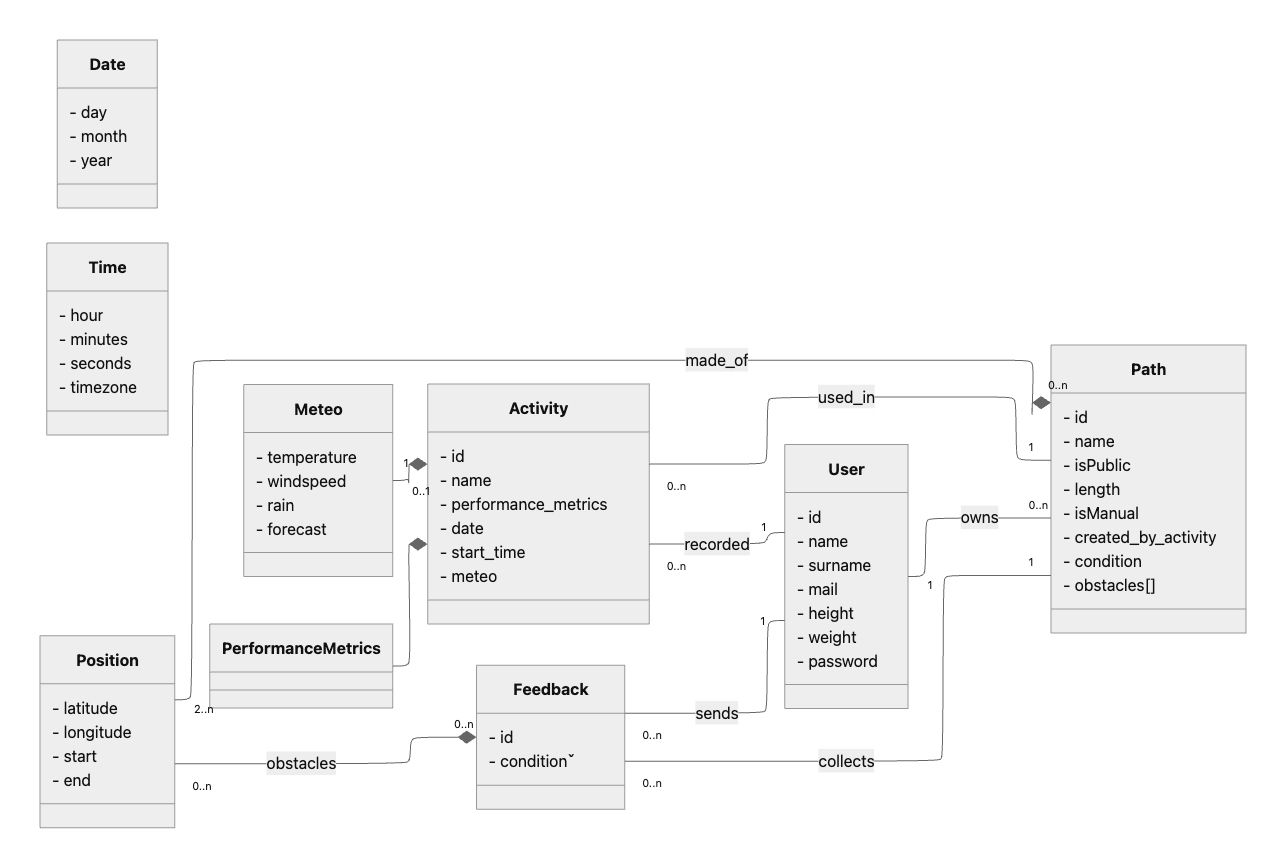
\includegraphics[width=0.9\textwidth]{Images/domain_class_diagram.jpeg}
    \caption{Domain Class Diagram}
    \label{fig:domain-class-diagram}
\end{figure}

The diagram illustrates the system's static structure:
\begin{itemize}
    \item \textbf{User:} The primary actor of the system. Beyond authentication credentials, this entity stores physical attributes (e.g. height, weight) essential for calculating performance metrics. The User acts as the owner of recorded \textbf{Activities}, created \textbf{Paths}, and submitted \textbf{Feedback}.
    \item \textbf{Path:} The core artifact, defined by metadata (e.g. isPublic) and a geometry composed of \textbf{Position} coordinates. It can be created manually or derived from an activity.
    \item \textbf{Activity:} Represents a tracking session with temporal data (e.g. start\_time), \textbf{PerformanceMetrics}, and \textbf{Meteo} conditions. It is linked to the User and optionally to a Path (used\_in).
    \item \textbf{Feedback:} Models user reports on path conditions. It references specific \textbf{Position} points to spatially locate obstacles (e.g., potholes) along the path's geometry.
    \item \textbf{Position:} The shared geospatial unit ensuring consistency between paths, traces, and feedback locations.
\end{itemize}


\subsection{State Diagrams}

\subsubsection*{Activity Recording}
\begin{figure}[H]
    \centering
    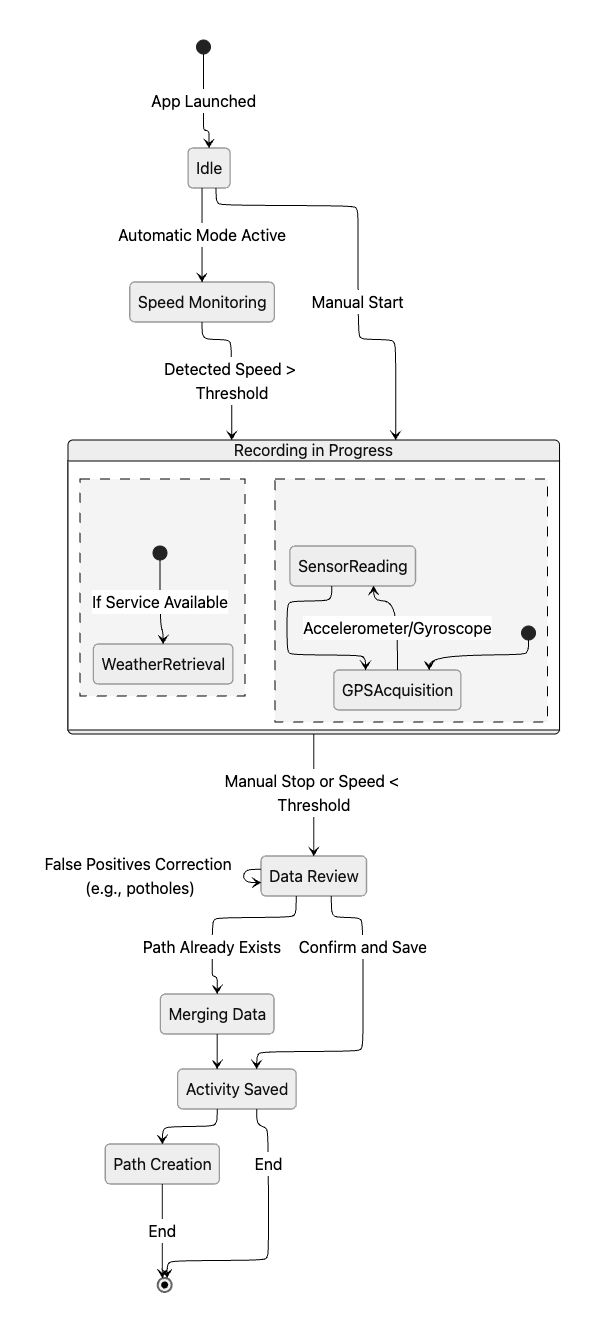
\includegraphics[width=0.5\textwidth]{Images/activity_recording_state_diagram.jpeg}
    \caption{Activity Recording State Diagram}
    \label{fig:activity-recording-state-diagram}
\end{figure}

This state machine describes the complete lifecycle of a cycling activity recording session.

The process begins in the \textbf{Idle} state. From here, the system can transition to the active phase in two distinct ways: \begin{itemize} \item \textbf{Manual Start:} The user explicitly initiates the session, moving directly to \textbf{Recording in Progress}. \item \textbf{Automatic Detection:} If "Automatic Mode" is active, the system enters the \textbf{Speed Monitoring} state. Upon detecting a speed greater than the predefined threshold, it automatically transitions to \textbf{Recording in Progress}. \end{itemize}

The \textbf{Recording in Progress} state is a composite state where the system continuously loops between \textbf{GPS Acquisition} and \textbf{Sensor Reading} (collecting data from the accelerometer and gyroscope). Concurrently, if the service is available, the system performs a \textbf{Weather Retrieval} operation to enrich the activity data.

The recording phase concludes when a "Manual Stop" occurs or the speed drops below the threshold, triggering a transition to the \textbf{Data Review} state. This is a mandatory validation phase where the user verifies the collected data and performs \textbf{False Positives Correction} (e.g., removing incorrectly detected potholes).

Once the review is confirmed, the system logic branches based on the GPS trace analysis: \begin{enumerate} \item \textbf{Merging Data:} If the system detects that the activity matches an existing public path, it transitions to this state to integrate the new feedback (obstacles/conditions) with the existing path data. \item \textbf{Direct Saving:} If no matching public path is found, the system proceeds directly to \textbf{Activity Saved}. \end{enumerate}

Both flows converge in the \textbf{Activity Saved} state. From here, the process either terminates or transitions to \textbf{Path Creation}, allowing the user to generate a new path entity from the recorded trace (a process detailed in a separate diagram).

\subsubsection*{Path Creation}
\begin{figure}[H]
    \centering
    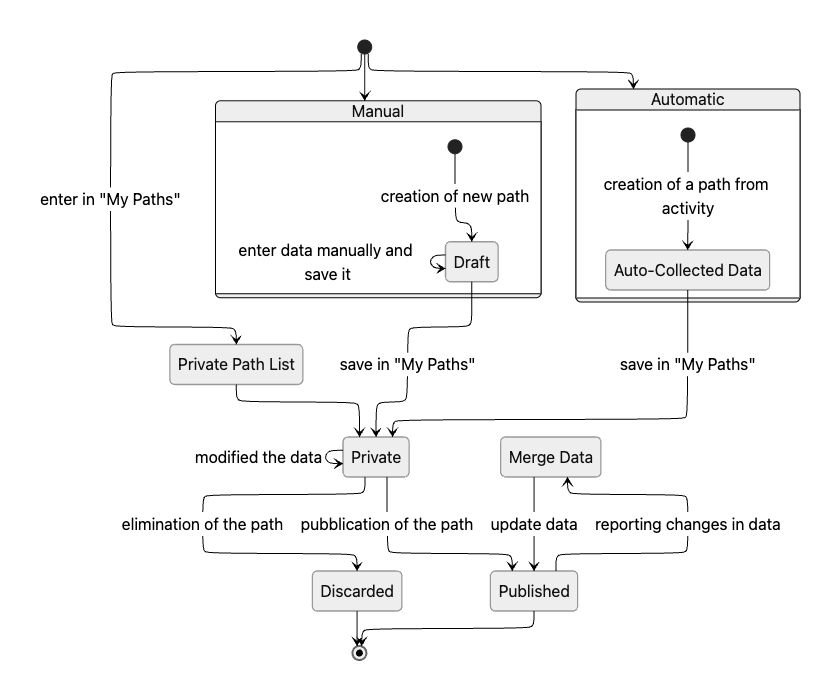
\includegraphics[width=0.9\textwidth]{Images/path_creation.jpeg}
    \caption{Path Creation State Diagram}
    \label{fig:path-creation-state-diagram}
\end{figure}
The diagram illustrates the creation, management, and evolution process of the Path object within the system. The lifecycle is divided into two macro-phases: instantiation (Manual or Automatic) and state management (Private or Public).
\begin{itemize}
    \item \textbf{Path Instantiation:}
    \begin{itemize}
        \item \textbf{Manual Creation:} The user enters the descriptive data of the path, which is initially managed in a draft state (Draft) within the Manual context. Upon saving, the path transitions to the user's personal list.
        \item \textbf{Automatic Creation:} The system generates the path based on data collected during a cycling activity (Auto-Collected Data). Once the acquisition is complete, the path is saved and persisted in the private section.
    \end{itemize}

    \item \textbf{Management and Publication:}
    \begin{itemize} 
        \item \textbf{Private State:} Once saved (or by accessing "My Paths"), the path resides in the \textbf{Private} state. In this phase, the user has full control over the entity: they can modify the data (modified the data cycle), permanently delete the path (transition to Discarded), or proceed to publication.
        \item \textbf{Published State:} Upon publication, the path becomes visible to the community. In this state, modifications are no longer direct but follow a collaborative process: users can report changes (reporting changes), which are processed by the system via the \textbf{Merge Data} function. This function validates and integrates the new information, triggering the actual update of the public data (update data).
    \end{itemize}
\end{itemize}


\subsubsection*{Meteorological Data Retrieval}
\begin{figure}[H]
    \centering
    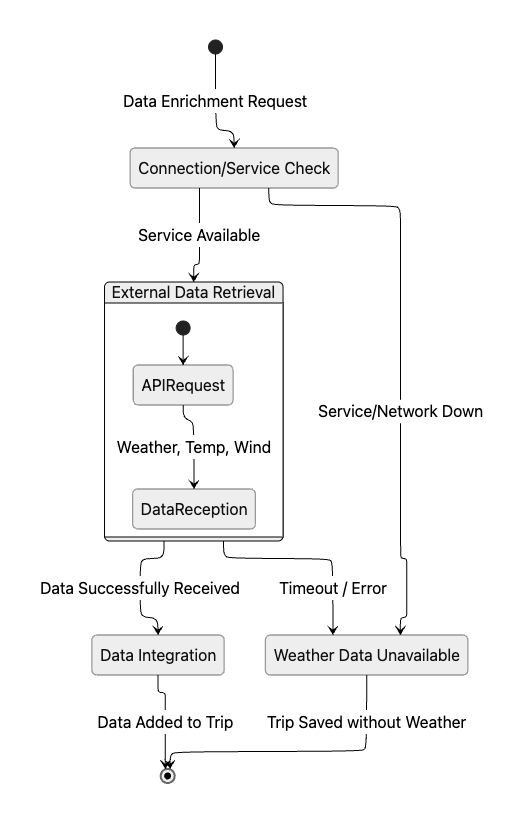
\includegraphics[width=0.5\textwidth]{Images/meteorological_data_state_diagram.jpeg}
    \caption{Meteorological Data Retrieval State Diagram}
    \label{fig:meteorological-data-retrieval-state-diagram}
\end{figure}
This diagram represents the enrichment of an activity with meteorological data.
If the device is connected to the network, a request is sent to an external API.
If the request is successful, the service retrieves data such as wind speed, temperature, and weather conditions, and formats them in a consistent way.
The system then embeds this information into the activity and saves it to the database.
If the request fails, the error is handled and the activity is saved without meteorological data.

\subsubsection*{Path Research}
\begin{figure}[H]
    \centering
    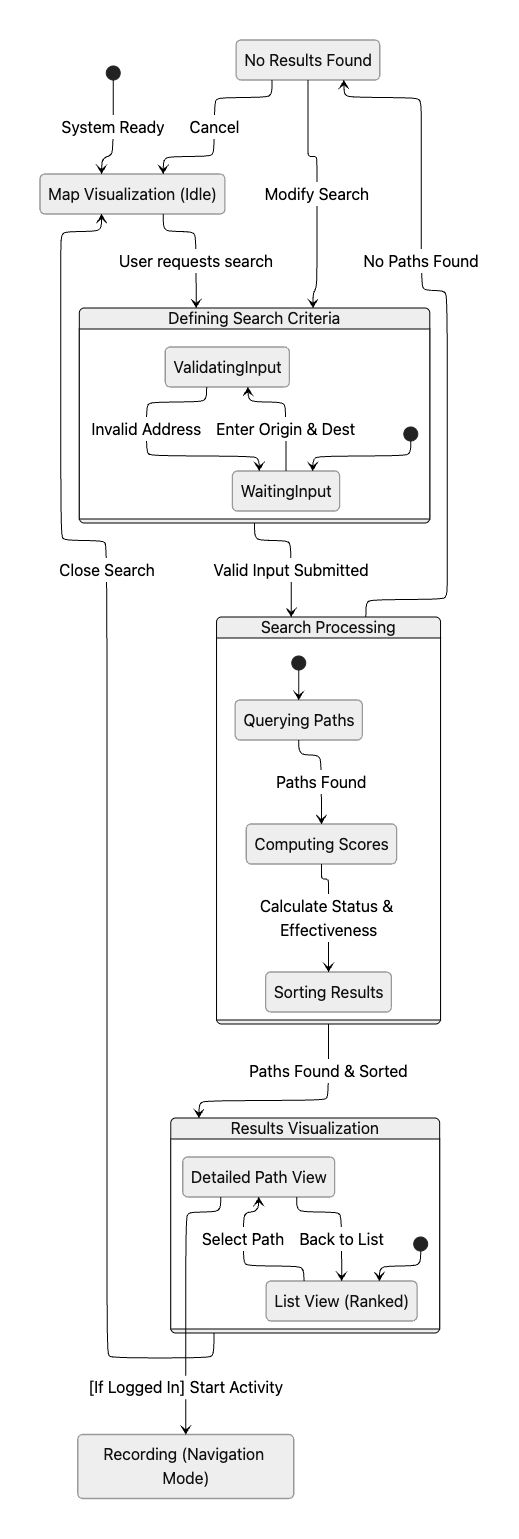
\includegraphics[width=0.4\textwidth]{Images/path_research_state_diagram.jpeg}
    \caption{Path Research State Diagram}
    \label{fig:path-research-state-diagram}
\end{figure}
This state machine describes the logic flow of the ``Path Search'' functionality, accessible to both Guest and Registered users.

The process begins in the \textbf{Map Visualization} state. When a user initiates a search, the system transitions to \textbf{Defining Search Criteria}, waiting for valid Origin and Destination inputs.

Upon submission, the system enters the \textbf{Search Processing} state. This is a critical system-side phase where three operations occur sequentially:

\begin{enumerate}
    \item \textbf{Querying Paths:} The system retrieves all geometrically valid paths between the two points.
    \item \textbf{Computing Scores:} The system calculates a specific score for each path, aggregating its maintenance status and its effectiveness in reaching the destination.
    \item \textbf{Sorting Results:} Paths are ranked based on the computed score.
\end{enumerate}

If valid paths exist, the system transitions to \textbf{Results Visualization}. Here, the user can toggle between a ranked list and a \textbf{Detailed Path View} (displaying specific obstacles, weather, and stats).

From the detailed view, a specific transition to \textbf{Recording (Navigation Mode)} is available, but guarded by the condition \texttt{[If Logged In]}, as only registered users can proceed to track an activity on the selected path.

\subsubsection*{User Lifecycle}
\begin{figure}[H]
    \centering
    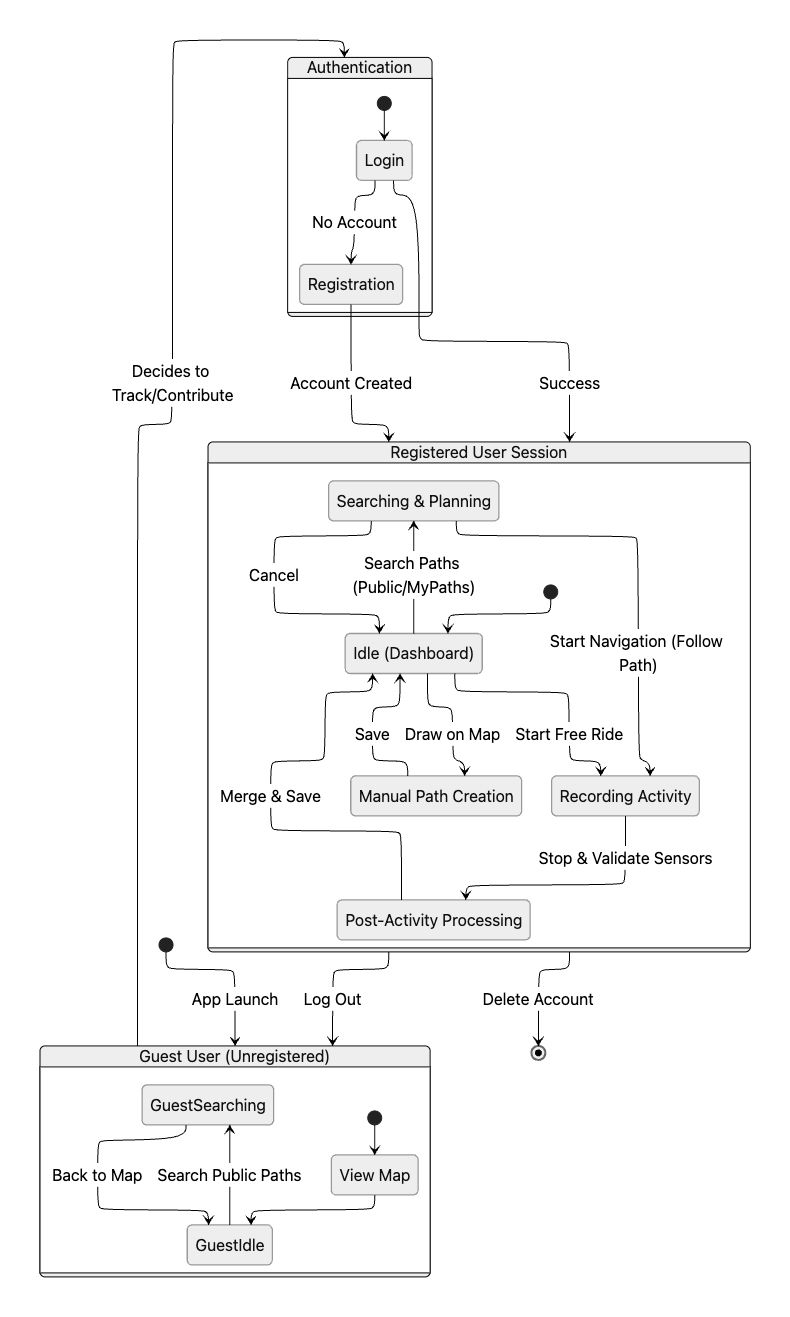
\includegraphics[width=0.6\textwidth]{Images/user_lifecycle_state_diagram.jpeg}
    \caption{User Lifecycle State Diagram}
    \label{fig:user-lifecycle-state-diagram}
\end{figure}

This state machine diagram describes the user lifecycle within the BBP system, distinguishing between two main macro-states: \textbf{Guest User}, unauthenticated, and \textbf{Registered User Session}, authenticated.

The lifecycle begins in the \textbf{Guest User} state, where functionalities are restricted to read-only operations (represented by the \textbf{Guest Searching} state). In this phase, the user can browse the public path inventory but cannot contribute data. To access active functionalities, a transition through the \textbf{Authentication} state (Login or Registration) is required.

Once authenticated, the user enters the composite \textbf{Registered User Session} state. Here, the \textbf{Idle} state acts as a central hub from which three main operational flows branch out:

\begin{enumerate}
    \item \textbf{Searching \& Planning:} The user searches for specific paths. From this state, the user can return to the Dashboard or transition directly to \textbf{Recording Activity}, following a selected path.
    \item \textbf{Recording Activity:} This represents the active cycling phase. It can be triggered via the search flow or directly from the Dashboard, not referring to any existing path.
    \item \textbf{Manual Path Creation:} The user enters an editor mode to manually trace routes on the map without physical recording.
\end{enumerate}
A critical transition occurs at the end of every recording session: the system moves to the \textbf{Post-Activity Processing} state. In this mandatory phase, the user validates sensor-detected data and the system executes the merging logic with the existing inventory before returning the user to the \textbf{Idle} state.
The lifecycle concludes when the user performs a logout or permanently deletes their account.